\chapter{Automatic Code Generation for RNA}
\label{cap:code_gen}

% Introduction

% TODO: move away from implementation/algorithm description

In this chapter, we present a mechanism for automatic code generation for the RNA Framework. This enables network operators to deploy the Framework without having the experience and knowledge to develop software for Zeek or programmable forwarding devices (P4). To support this mechanism, in the previous chapter, we proposed additions to the RNA Framework.

Before we talk about the mechanism behind the RNA automation, it is important to clarify the idea of offloading Zeek Scripts. When we talk about offloading scripts, we are not offloading the processing of the scripts that happen on the PSI (see Section \ref{sec:bg:zeek_psi}). We offload the steps and procedures required to transform network packets into the structures that are needed to run these scripts, usually Zeek Events. Those operations selected for offloading, which are described in Section \ref{sec:bg:zeek_candidate_operations} and also analyzed in-depth by \citeonline{Ilha2022}, make the system more performative and able to support more network throughput in this world of constantly increasing network speeds.

This automation mechanism started with the idea of having a set of Zeek scripts as input, and two components on the output: a Zeek Script/Package and a P4 program. This became evidently unfeasible for the scope of this project due to the complexity and the logic behind each event triggering logic in Zeek. This obstacle steered us into another approach. The proposed mechanism uses both previously mentioned concepts, the \ProtocolTemplates{} and the \Offloaders{}, as a source of templates and resources, in order to implement the software required to offload the desired scripts. Another proposed change to the design is the generation of a unique Zeek Plugin, which will automatically deploy the P4 code when initiated, instead of having two separate deployable components.

\section{Overview}
\label{sec:code_gen:overview}

This section presents an overview of the RNA Code Generation Mechanism, starting with its inputs and expected output, which is illustrated in Figure \ref{fig:code_gen_black_box}. The main input for this tool is the set of scripts to be offloaded. These scripts need to be given in full, including their source code so the Tool can extract what events they monitor.

\begin{figure}[htb]
    \caption{RNA - Code Generator Mechanism - Inputs and Outputs}
    \begin{center}
        \includegraphics[width=0.98\textwidth]{images/code_gen_black_box.pdf}  
    \end{center}
    \label{fig:code_gen_black_box}
    \legend{Source: the author}
\end{figure}

The second set of inputs are what we call templates, both \ProtocolTemplates{} and \Offloader{} Templates. They are a pool of known implementations of protocols and events that can be used for offloading scripts. A template being present in this pool doesn't mean it will be included in the final output, but it means it is available in case a script needs its implementation.

The desired output of our Tool is a single Zeek Plugin following the structure previously presented in Section \ref{sec:rna:overview} and illustrated in Figure \ref{fig:arch_low_level}. This Zeek Plugin when executed should: configure the switch, create a mirroring session for the Zeek monitoring system, deploy the P4 code, and register all Translators in Zeek's Event Engine. This eliminates the need for the operator to coordinate the deployment of two separate systems, the RNA Host Engine, and the RNA Switch Engine.

To be able to execute this task, the first objective of the RNA Tool is to analyze all the provided Zeek scripts and identify which are the observed events in every script. Once this pool of events is created, the pool selects \Offloaders{} (from the templates pool) are capable of offloading those events. This step is finished and succeeds if all events are capable of been offloaded. It is also important to note that one Offloader may offload more than one event at a time, which can be an advantage, lowering the number of \Offloaders{} per deployment.

After all events and \Offloaders{} have been selected, the mechanism must ensure all templates for the protocols required by these \Offloaders{} are available. After all this knowledge model is complete, the mechanism generates all required source files.

Some of the resulting code that is present in the final Zeek Plugin is extracted and merged from the templates, and not completely generated by our tool. It is not yet possible to fully generate all offloader code, because the process of converting C++ or P4 code from one to another is very complicated and is out of the scope of this project. As explained in the previous section, while our code generator is not able to fully generate all required code, some of it must be included in the templates.

\section{Detailed Mechanism Design}
\label{sec:code_gen_impl}

The operation of our RNA Code Generation Mechanism can be classified into two different stages. The first stage is building our knowledge model, which include all Protocol Templates, \Offloaders{}, events and scripts desired by the network operator. We call this knowledge model \textit{ProtocolGraph}. The second stage is the actual code merge and generation using this structured and validated knowledge model from the previous step. We start this section explaining the first stage of our prototype, the process of building our \textit{ProtocolGraph}.

\subsection{Knowledge Model}

The core logic behind the implementation of our RNA Code Generation Mechanism relies on a structure we call \textit{ProtocolGraph}. This structure stores in a graph structure all protocols required for our events of interest. The \Offloaders{} are linked to their final protocol level in the graph, generating us a structure as presented in Figure \ref{fig:protocol_graph}.

\begin{figure}[htb]
    \caption{Knowledge Model - Protocol Graph}
    \begin{center}
        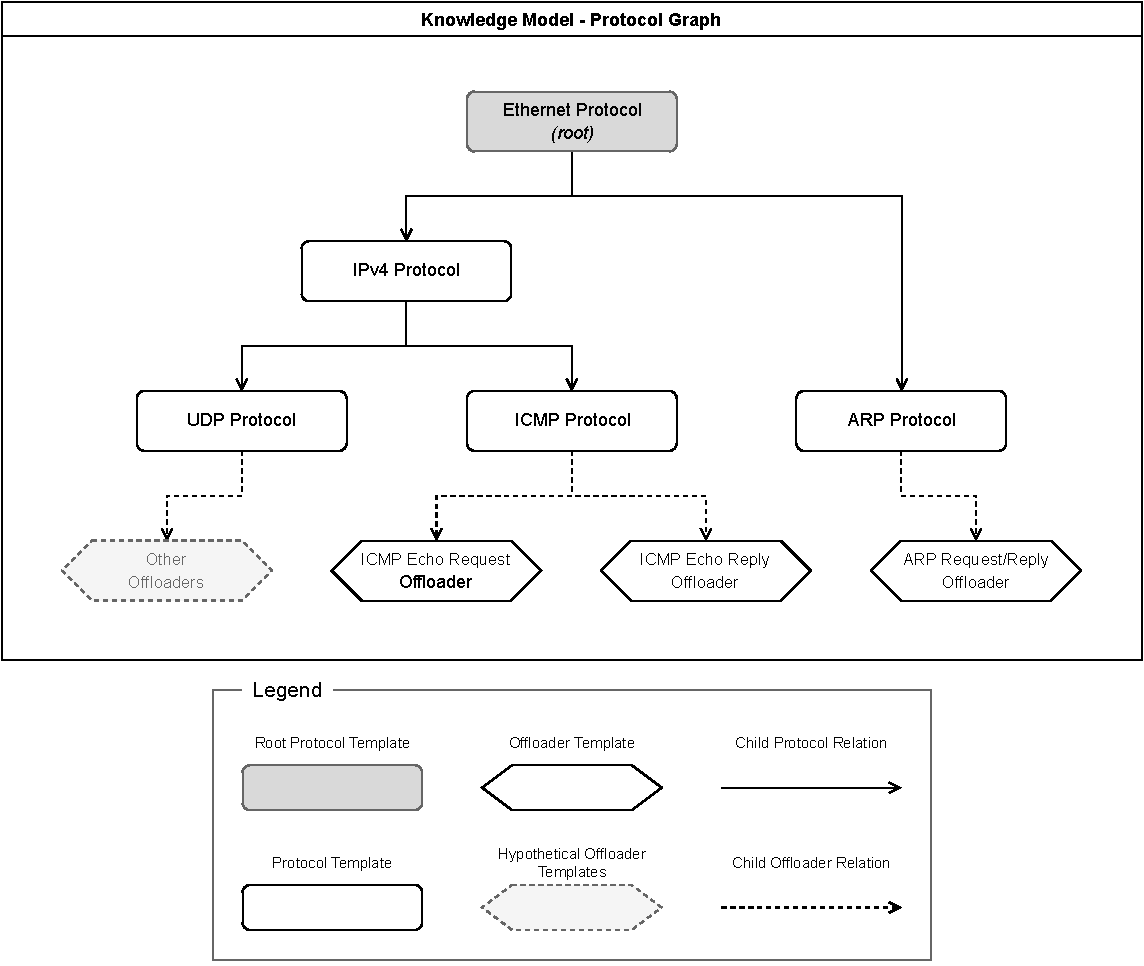
\includegraphics[width=0.98\textwidth]{images/icmp_ex_protocol_graph.pdf}  
    \end{center}
    \label{fig:protocol_graph}
    \legend{Source: the author}
\end{figure}

% def build(self):
%     """Builds the graph and validates it.
%     """
%     self._validate_component_list(self.raw_components)

%     protocol_list = _filter_list_by_type(
%         self.raw_components, ProtocolComponent)
%     offloader_list = _filter_list_by_type(
%         self.raw_components, OffloaderComponent)

%     self.required_offloaders = self._get_required_offloaders(offloader_list)

%     if len(self.required_offloaders) == 0:
%         raise ZpoException("No Offloader or Zeek Event specified for offloading. Aborting.")

%     # Remove not required offloaders
%     offloader_list = _filter_list(
%         lambda offloader: offloader.id in self.required_offloaders, offloader_list)

%     self.protocols: Dict[str, ProtocolComponent] = _make_template_dict(
%         protocol_list)
%     self.offloaders: Dict[str, OffloaderComponent] = _make_template_dict(
%         offloader_list)

%     self.root = self._find_root_protocol()

%     self._link_graph()
%     self._attach_offloaders()
%     self._check_for_cycles()
%     self._trim_unused_protocols()
%     self._remove_unreachable_protocols()

%     self._set_protocol_depths()
%     self._sort_protocols()
%     self._sort_offloaders()
%     self._set_offloaders_uids()

%     self.is_built = True
% Describe how to actually works and maybe some implementation details


\subsection{Code Generation}